\documentclass{beamer}
\usepackage{amsmath}
\usepackage{amssymb}
\usepackage{pgf}
\usepackage{tikz}
\usepackage{listings}
\usepackage{color}
\usetikzlibrary{matrix}
\usetheme{boxes}
\newcommand{\fig}{./figures} % common figure path
\newcommand{\dbbslsh}{\textbackslash \textbackslash} % common figure path
\newenvironment{myblock}[3]{%
\definecolor{smtbx}{rgb}{0.64,0.76,0.68}
\setbeamercolor{block body}{#2}
\setbeamercolor{block title}{#3}
\begin{block}{#1}}{\end{block}}
\newcommand{\frnzplt}{FranzPlot }
\DeclareMathSymbol{\shortminus}{\mathbin}{AMSa}{"39}

\title[Curve e Sup. - Lab 3]{Curve e Superfici per il Design \\ Laboratorio - 3}
\author[Prof. Parolini]{Prof. Nicola Parolini}
%\institute[dimat]{Long Inst.}
\date{7 Novembre 2019}

\begin{document}

\begin{frame}
\frametitle{Materiali}
Il materiale per l'esercitazione di oggi:
\begin{itemize}
\item Questa presentazione \\ (\texttt{Materiale Didattico/Laboratori/lab 4/lab4\_testo.pdf});
%\item Il file \texttt{es\_dado\_ref.toml} con l'esercizio risolto della passata esercitazione.
\item L'eseguibile del \frnzplt \\ (\texttt{Software/Franzplot 19.08 - Windows.exe})
\end{itemize}
\end{frame}

Per il calcolo della rappresentazione parametrica di una retta abbiamo bisogno di
un punto per cui passa la retta e di un vettore direttore.

\section{Esercizi}
\begin{frame}
\frametitle{Esercizio 1}
Dati i punti
$$
\mathbf{P}=\left[
\begin{array}{c}
0\\
-2\\
-1
\end{array}
\right]
\qquad
\mathbf{R}=\left[
\begin{array}{c}
3\\
-1\\
2
\end{array}
\right] \qquad
\mathbf{S}=\left[
\begin{array}{c}
-2\\
1\\
0
\end{array}
\right] 
$$
si calcolino:
    \begin{itemize}
    \item una rappresentazione parametrica della retta $r$ \\ passante per $\mathbf{P}$ e $\mathbf{R}$.
    \item una rappresentazione parametrica della retta $s$ \\ passante per $\mathbf{P}$ e $\mathbf{S}$.
    \end{itemize}
    
Le due rette sono perpendicolari?
\end{frame}

\begin{frame}
\frametitle{Esercizio 1 - i}

La rappresentazione di $r$ e $s$ non sono uniche; la pi\`u immediata per $r$ sar\`a:
\begin{itemize}
        \item vettore direttore $\overrightarrow{PR}$
        \item retta passante per $P$
\end{itemize}
Dai dati ricaviamo che:
$$
\overrightarrow{PR} = \left[
\begin{array}{c}
3\\
1\\
3
\end{array}
\right]
\qquad
\mathbf P = \left[
\begin{array}{c}
0\\
-2\\
-1
\end{array}
\right]
$$
quindi 
$$r: \quad \left\{
\begin{array}{rcl}
x&=&3t+0\\
y&=&1t-2\\
z&=&3t-1
\end{array}
\right. \quad t\in \mathbb{R}
$$
\end{frame}

\begin{frame}
\frametitle{Esercizio 1 - ii}

Alla stessa maniera, per $s$ scegliamo:
\begin{itemize}
        \item vettore direttore $\overrightarrow{PS}$
        \item retta passante per $P$
\end{itemize}
Dai dati ricaviamo che:
$$
\overrightarrow{PS} = \left[
\begin{array}{c}
-2\\
3\\
1
\end{array}
\right]
\qquad
\mathbf P = \left[
\begin{array}{c}
0\\
-2\\
-1
\end{array}
\right]
$$
quindi 
$$s: \quad \left\{
\begin{array}{rcl}
x&=&\shortminus 2t+0\\
y&=&\ 3t-2\\
z&=&\ 1t-1
\end{array}
\right. \quad t\in \mathbb{R}
$$

Nota: le rappresentazioni non sono uniche! Esempio: come termine noto
per $r$ avremmo potuto usare il punto $\mathbf R$, e per $s$ il punto $\mathbf S$.
\end{frame}

\begin{frame}
\frametitle{Esercizio 1-ii}
Affinch\'e due rette siano perpendicolari, esse devono essere incidenti e le loro direzioni
devono formare un angolo retto.

    \vspace{0.4cm}
In questo caso sappiamo gi\`a che le rette hanno il punto $\mathbf P$ in comune, quindi sappiamo
che sono incidenti. Verifichiamo se le direzioni formano un angolo retto:
\begin{displaymath}
\overrightarrow{PR} \cdot \overrightarrow{PS}
    =
\begin{bmatrix} 3 \\ 1 \\3 \end{bmatrix}\cdot \begin{bmatrix}\shortminus 2\\ 3 \\1 \end{bmatrix} =
    \shortminus 6 + 3 + 3 = 0
\end{displaymath}

Possiamo quindi concludere che le rette sono perpendicolari.
\end{frame}

    
%
%
\begin{frame}
\frametitle{Esercizio 2}
\begin{itemize}
\item Rappresentare la retta $r$ passante per i punti
\begin{displaymath}
\mathbf{P}=\begin{bmatrix}2\\1\\1 \end{bmatrix},\;\;\;\;\;
\mathbf{Q}=\begin{bmatrix}1\\1\\3 \end{bmatrix};
\end{displaymath}
\item Determinare la retta $s$ perpendicolare ad $r$ e passante per:
\begin{displaymath}
\mathbf{M}=\begin{bmatrix}1\\2\\-2 \end{bmatrix}.
\end{displaymath}
\end{itemize}
\end{frame}

\begin{frame}
\frametitle{Esercizio 2 - i}
\begin{columns}
\begin{column}{0.48\textwidth}
\begin{itemize}
\item Vettore direttore \\ della retta $r$:
\end{itemize}
\end{column}
\begin{column}{0.58\textwidth}
\begin{displaymath}
\overrightarrow{PQ} =\begin{bmatrix}\shortminus 1 \\ 0 \\ 2 \end{bmatrix}
    \quad
    \mathit{oppure}
    \quad
\overrightarrow{QP} =\begin{bmatrix}1 \\0 \\ \shortminus 2 \end{bmatrix}
\end{displaymath}
\end{column}
\end{columns}
\begin{columns}
\begin{column}{0.58\textwidth}
\begin{itemize}
\item Rappresentazione della retta $r$:
\end{itemize}
\end{column}
\begin{column}{0.48\textwidth}
\begin{displaymath}
r :\begin{cases} x = -t +1\\ y = 1 \\z = 2t+3 \end{cases}
\end{displaymath}
\end{column}
\end{columns}

\end{frame}

\begin{frame}
\frametitle{Esercizio 2 - ii}
Se voglio trovare una retta perpendicolare a $r$ che passa per $\mathbf M$, devo trovare un punto
$\mathbf H \in r$ tale che $\overrightarrow{MH} \perp \overrightarrow{PQ}$

\vspace{0.4cm}
    $\mathbf H$ incognito, so solo che appartiene a $r$!
\begin{itemize}
    \item ma se appartiene a $r$, allora $\mathbf H = r(\tilde{t})$
    \item $\mathbf H :\begin{cases} \mathbf H_x = -\tilde t +1\\ \mathbf H_y = 1 \\ \mathbf H_z = 2 \tilde t+3 \end{cases}$
\end{itemize}

\vspace{0.4cm}
$$
\overrightarrow{MH}
    =
    \mathbf H - \mathbf M
    =
    \begin{bmatrix}\shortminus \tilde t + 1\\ 1 \\ 2 \tilde t+3 \end{bmatrix} - \begin{bmatrix}1 \\ 2 \\ \shortminus 2 \end{bmatrix}
    =
    \begin{bmatrix}\shortminus \tilde t \\ \shortminus 1 \\ 2 \tilde t+5 \end{bmatrix}
$$
\end{frame}

\begin{frame}
\frametitle{Esercizio 2 - iii}
\begin{displaymath}
\overrightarrow{MH} \perp \overrightarrow{PQ} 
    \Rightarrow  
\overrightarrow{MH} \cdot \overrightarrow{PQ} = 0  
\end{displaymath}
Scritto in forma vettoriale:
$$
    \begin{bmatrix}\shortminus \tilde t \\ \shortminus 1 \\ 2 \tilde t+5 \end{bmatrix}
        \cdot
    \begin{bmatrix}\shortminus 1 \\ 0 \\ 2 \end{bmatrix} = 0
$$
Svolgo il prodotto scalare, ottengo una equazione in $\tilde t$
$$
    \tilde t + 0 + 4 \tilde t + 10 = 0 \quad \Rightarrow \quad 5 \tilde t = \shortminus 10
$$
    Quindi, il valore del parametro che cercavo \`e $\tilde t = \shortminus 2$!
\end{frame}

\begin{frame}
\frametitle{Esercizio 2 - iv}
Il problema richiedeva di trovare una parametrizzazione di $s$. Scegliamo:
\begin{itemize}
        \item vettore direttore $\overrightarrow{MH}$
        \item retta passante per $M$
\end{itemize}

Per trovare i valori del vettore $\overrightarrow{MH}$, vado a sostituire il valore ricavato
per $\tilde t$:
$$
\overrightarrow{MH}
    =
    \begin{bmatrix}\shortminus \tilde t \\ \shortminus 1 \\ 2 \tilde t+5 \end{bmatrix}
\Rightarrow
\tilde t = \shortminus 2
\Rightarrow
\overrightarrow{MH}
    =
    \begin{bmatrix}2 \\ \shortminus 1 \\ 1\end{bmatrix}
        \qquad
    \mathbf M
    =
    \begin{bmatrix}1 \\ 2 \\ \shortminus 2 \end{bmatrix}
$$
\begin{columns}
\begin{column}{0.48\textwidth}
\begin{itemize}
\item Sostituisco nell'espressione per $s(t)$, trovando:
\end{itemize}
\end{column}
\begin{column}{0.48\textwidth}
\begin{displaymath}
s:
\begin{cases}
x  = 2t + 1 \\
y  = \shortminus t  + 2 \\
z  = \ t  - 2
\end{cases}
\end{displaymath}
\end{column}
\end{columns}
\end{frame}
%

\begin{frame}
\frametitle{Esercizio 2 - iv}
\begin{center}
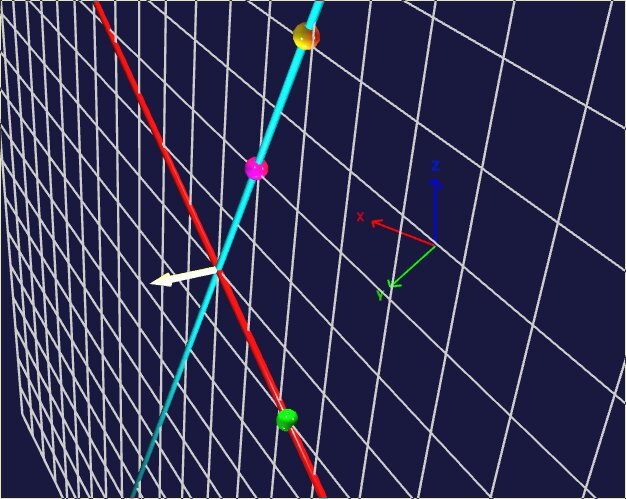
\includegraphics[width = 0.9\textwidth]{\fig/l4_es2.jpeg}
\end{center}
\end{frame}
%
\begin{frame}
\frametitle{Esercizio 3 - i}
Con \frnzplt \`e possibile rappresentare un piano parametricamente, come una superficie qualsiasi.
\begin{itemize}
\item Rappresentare la retta $r$:
\begin{displaymath}
r:\begin{cases}
x = t \\
y = 0.5~t\\
z = 0
\end{cases}
\end{displaymath}
\item Rappresentare l'oggetto che si ottiene: 
\begin{enumerate}
\item Traslando la retta in direzione $y$ facendo variare il parametro della traslazione tra -5 e 5.
\item Ruotanto rispetto a z la retta di $2\pi$ radianti.
\end{enumerate}
\end{itemize}
\end{frame}
\begin{frame}
\frametitle{Esercizio 3 - ii}
\begin{center}
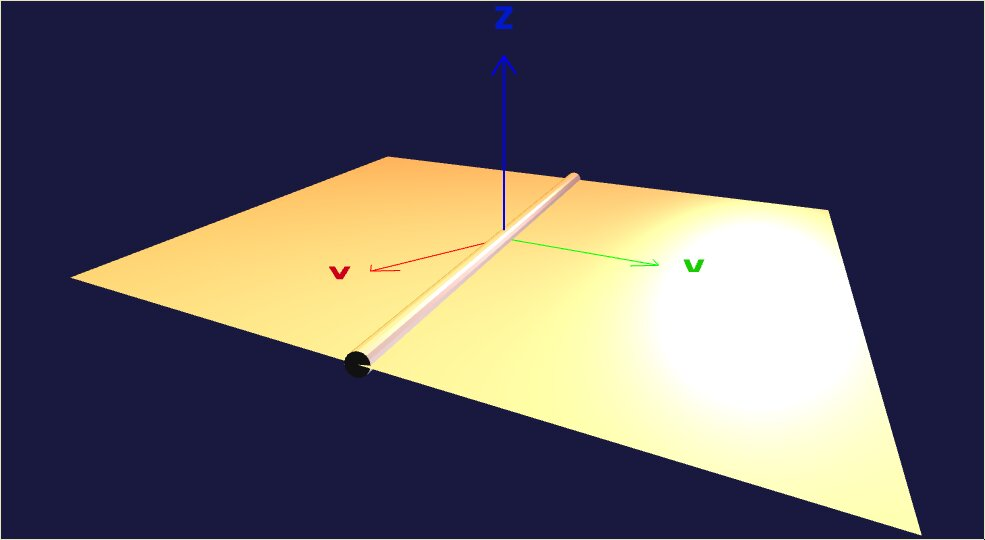
\includegraphics[width=0.5\textwidth]{\fig/l4_es3a.jpeg}
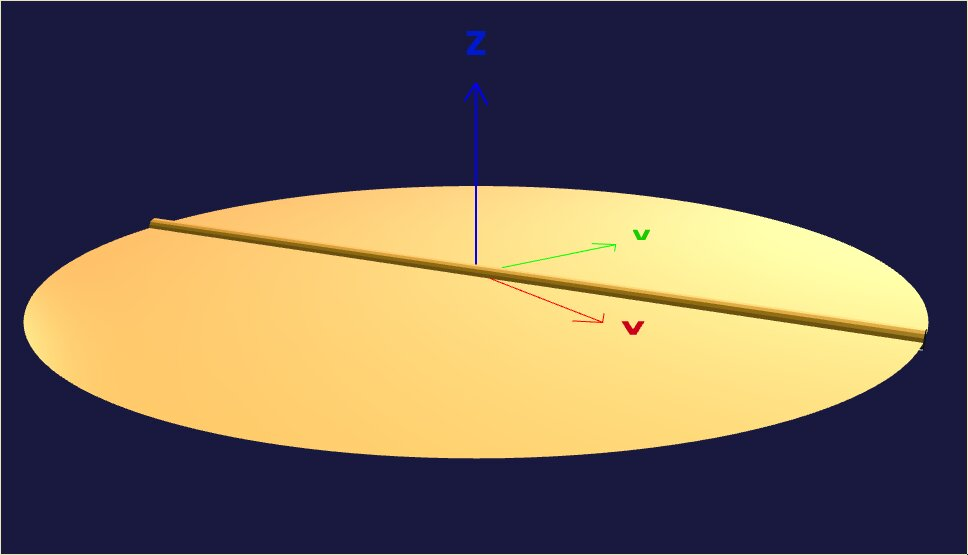
\includegraphics[width=0.5\textwidth]{\fig/l4_es3b.jpeg}
\end{center}
\end{frame}
\begin{frame}
\frametitle{Esercizio 4 - i}
Date le rette:
\begin{columns}

\begin{column}{0.33\textwidth}
\begin{displaymath}
p:\begin{cases} 
x = 3~t - \frac{1}{2}\\
y = t - \frac{1}{2}\\
z = -2~t
\end{cases}
\end{displaymath}
\end{column}
\begin{column}{0.33\textwidth}
\begin{displaymath}
q:\begin{cases} 
x = t - 13 \\
y = 2\\
z = -t + 15
\end{cases}
\end{displaymath}
\end{column}
\begin{column}{0.33\textwidth}
\begin{displaymath}
r:\begin{cases} 
x = t + \frac{3}{2}\\
y = t + \frac{1}{2}\\
z = 2~t -2
\end{cases}
\end{displaymath}
\end{column}
\end{columns}
\begin{itemize}
\item Rappresentare le rette con \frnzplt
\item Le rette $p$ e $q$ sono perpendicolari? E le rette $p$ ed $r$?
\item Determinare e rappresentare i punti di intersezione se presenti
\end{itemize}
\end{frame}
\begin{frame}
\frametitle{Esercizio 4 - ii}
\begin{itemize}
\item Scrivere l'equazione del piano $\alpha$ con normale $\mathbf{n}=[1,1,1]^T$ passante per il punto $(1,0,0)$. Rappresentare il piano con \frnzplt
\item Calcolare  e rappresentare i punti di intersezione di $p$ e $q$ con il piano.
\item Calcolare e rappresentare il piano $\beta$ su cui giacciono  le rette $p$ e $q$, e  scrivere l'espressione parametrica della retta $s$ intersezione dei piani $\alpha$ e $\beta$ 
\end{itemize}
\end{frame}
\begin{frame}
\frametitle{Esercizio 4 - iii}
\begin{center}
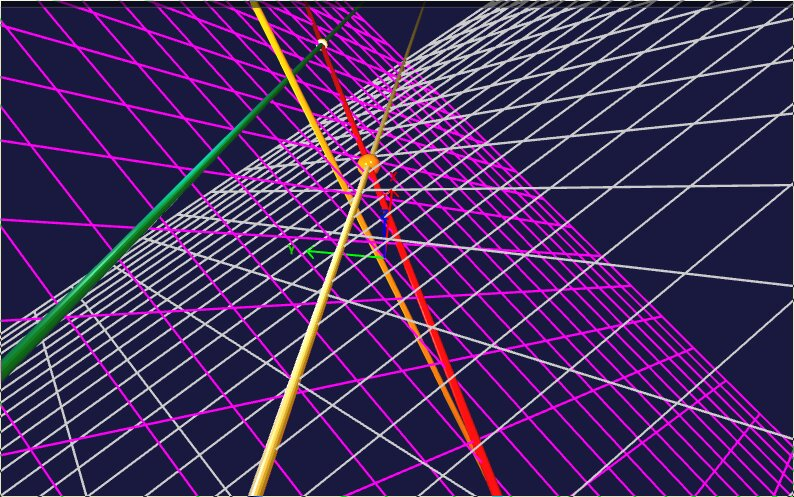
\includegraphics[width=0.9\textwidth]{\fig/l4_es5final.jpeg}
\end{center}
\end{frame}

\end{document}
